\section{Etherless-cli}	

	\subsection{Overview}
	The purpose of this module is to allow the end user to interact with the \textit{Etherless} platform. The module provides a set of commands that allows both the management of the Ethereum wallet and the interaction with smart contracts.
	
	\subsection{Architecture}
		\subsubsection{Commands}
		Package used to manage commands provided by the CLI.
		\begin{figure} [H]
			\centering
			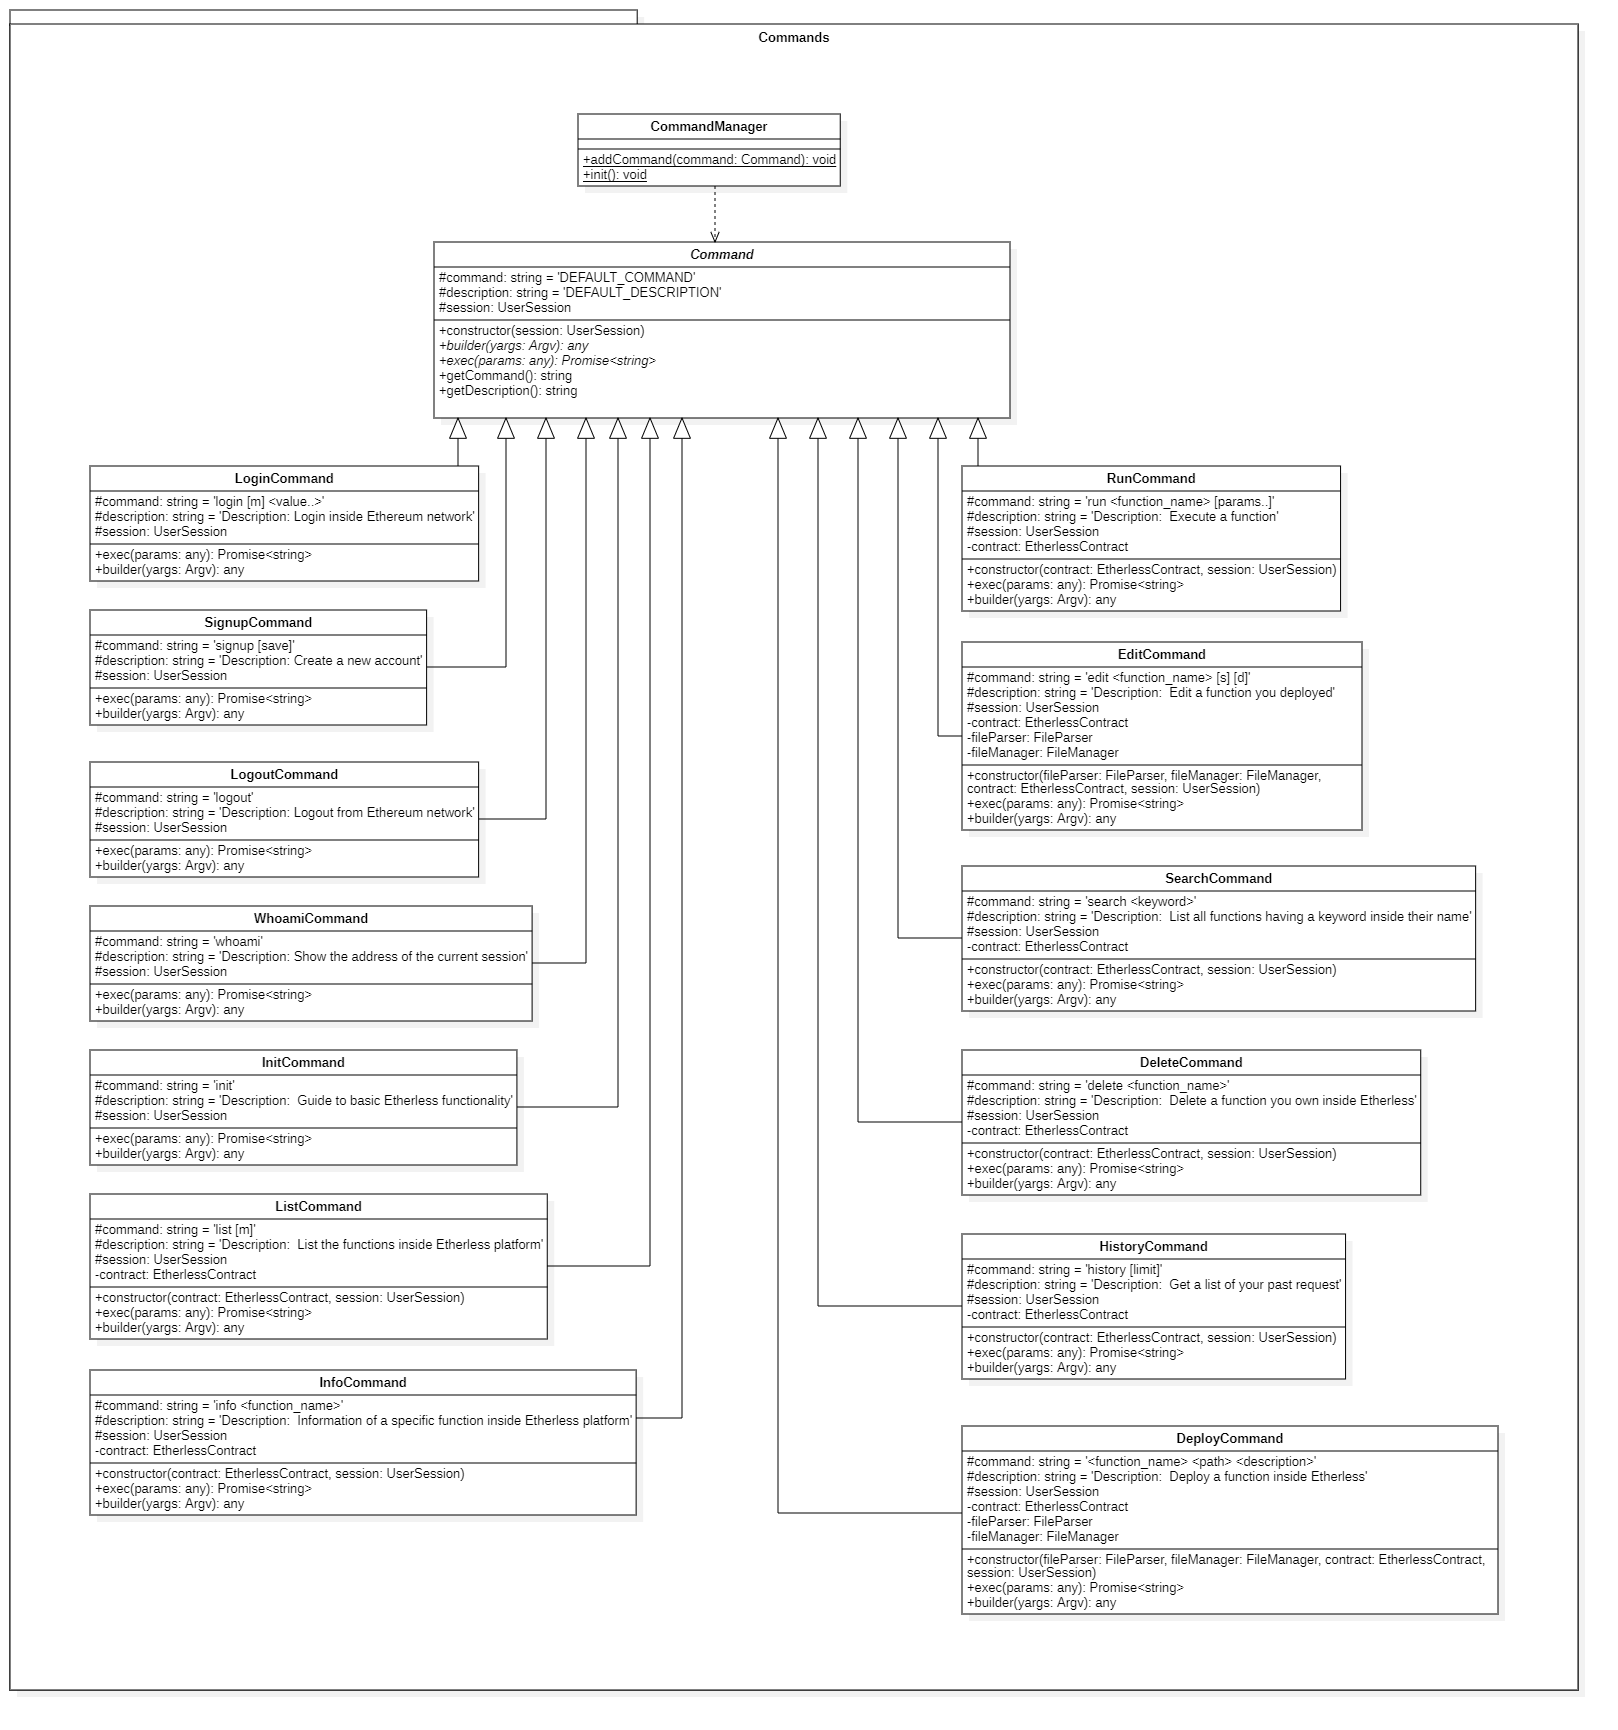
\includegraphics[width=0.6\linewidth]{diagrammi/etherless-cli/Commands}
			\caption{Class diagram of the Commands package.}
		\end{figure}
	
			\subsubsubsection{Command}
			Abstract class that describes the functionalities and attributes that every CLI command must have. To add any command to the CLI the developer needs to extend the Command class and implements the exec and builder methods. \\ 
			The command constructor exposes the dependecy from UserSession, making possible to  easily create mock objects of this class. 
			
				\subsubsubsection*{Attributes}
					\begin{itemize}
						\item \textbf{command}: syntax of the CLI command;
						\item \textbf{description}: a brief description of the command;
						\item \textbf{session}: UserSession object, used by the command to obtain information about the current user.
					\end{itemize}
				
				\subsubsubsection*{Methods} 
					\begin{itemize}
						\item \textbf{exec}: execute the specified command, it returns a string that will be shown to the user;
						\item \textbf{builder}: function that describes the details of the command parameters, such as position and expected type;
						\item \textbf{getCommand}: returns the command syntax for the CLI;
						\item \textbf{getDescription}: returns the command description.
					\end{itemize}
	
			\subsubsubsection{CommandManager} 
			This class is a collection of static methods needed to interact with the external library Yargs, used for command management. It exposes functionalities to add a new command and start processing user input. 
				\subsubsubsection*{Methods}
					\begin{itemize}
						\item \textbf{addCommand}: add a new command to the list of available CLI commands;
						\item \textbf{init}: start processing the user input.
					\end{itemize}
			
			\subsubsubsection{Implemented commands}
			\begin{itemize}
				\item \textbf{LoginCommand}: this class implements the login command, it allows the user to login inside the Ethereum network with both private key and mnemonic phrase; 
				\item \textbf{SignupCommand}: this class implements the signup command, it allows the user to create a new wallet inside Ethereum network; 
				\item \textbf{LogoutCommand}: this class implements the logout command, deleting all user credentials from the system;  
				\item \textbf{WhoamiCommand}: this class implements the whoami command, it allows the user to see his wallet address; 
				\item \textbf{InitCommand}: this class implements the init command, it allows the user to see a brief introduction of the application and informations about the authentication procedure; 
				\item \textbf{RunCommand}: this class implements the run command, it allows the user to execute a function inside \textit{Etherless} platform; 
				\item \textbf{EditCommand}: this class implements the edit command, it allows the user to modify the description or the source code of an owned function; 
				\item \textbf{SearchCommand}: this class implements the search command, it allows the user to get a list of all functions that contains the given keyword inside their name; 
				\item \textbf{InfoCommand}: this class implements the info command, it allows the user to get details about a function; 
				\item \textbf{DeleteCommand}: this class implements the delete command, it allows the user to delete an owned function; 
				\item \textbf{HistoryCommand}: this class implements the history command, it allows the user to see his past run requests;
				\item \textbf{DeployCommand}: this class implements the deploy command, it allows the user to deploy a function to the \textit{Etherless} platform.
			\end{itemize}
		
		\subsubsection{FParser}
 		This package is used to define all the classes and interfaces to manage source file parsing.
		
		\begin{figure} [h!]
			\centering
			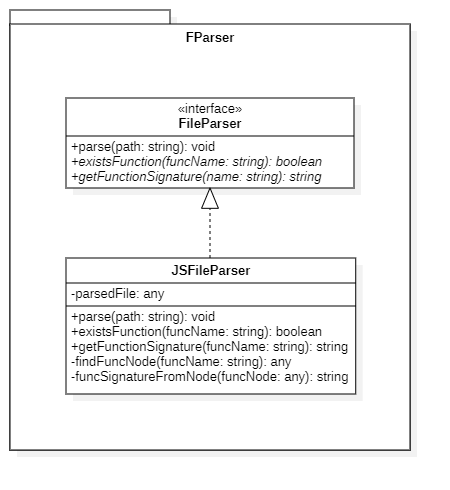
\includegraphics[width=0.5\linewidth]{diagrammi/etherless-cli/FParser}
			\caption{Class diagram of the FParser package.}
		\end{figure}
		
			\subsubsubsection{FileParser} 
			Interface used to define all methods needed for source file parsing. In particular the class focuses on methods needed to find function signature in source file. 
		
				\subsubsubsection*{Methods}
					\begin{itemize}
						\item \textbf{parse}: parses a file;   
						\item \textbf{existsFunction}: checks if the function with the given name exists inside the considered source file;
						\item \textbf{getFunctionSignature}: returns the signature of the function with the given name.
					\end{itemize}
		
			\subsubsubsection{JSFileParser}
			Since we manage the deploy only of Javascript source file, we created the class JSFileParser, that implements the interface FileParser. This class is mainly used to check if a function exists inside a source file, and to obtain its signature. To manage the Javascript source file parsing process we use the \texttt{acorn} library. 
			
				\subsubsection*{Attributes}
					\begin{itemize}
						\item \textbf{parsedFile}: tree structure created after the parsing process by the library \texttt{acorn}.
					\end{itemize}
				
				\subsubsection*{Methods}
				The class implements all methods defined in the FileParser interface, its defines also the following private methods: 
				\begin{itemize}
					\item \textbf{findFuncNode}: method used to find the node inside parsedFile attribute that refers to a function with a given name; 
					\item \textbf{funcSignatureFromNode}: method that extracts from a node of the parsedFile attribute the information about the function signature. 
				\end{itemize}
			
		\subsubsection{FManager} 			
		This package is used to define all the classes and interfaces used to manage file saving and retriving processes.
		\begin{figure} [h!]
			\centering
			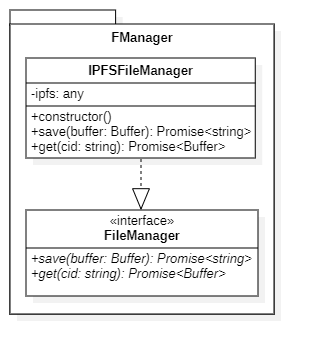
\includegraphics[width=0.5\linewidth]{diagrammi/etherless-cli/FManager}
			\caption{Class diagram of the FManager package.}
		\end{figure}	
				
			\subsubsubsection{FileManager}
			Interface that defines methods needed for saving and retriving files. 
		
				\subsubsubsection*{Methods}
					\begin{itemize}
						\item \textbf{save}: saves a file using a specific protocol;
						\item \textbf{get}: retrives information of a file.
				\end{itemize}
			
			\subsubsubsection{IPFSFileManager}
				Since we use the IPFS protocol to send and retrive file, we created the class IPFSFileManager, that implements the FileManager interface. To estabilish a connection to the IPFS network we use a small package, that is responsible for the hiring of the IPFS connection implementation (\texttt{ipfs-mini} API). 
				
				\subsubsubsection*{Attributes}
				\begin{itemize}
					\item \textbf{ipfs}: object through which the class can interact with the \texttt{ipfs-mini} API.
				\end{itemize}
				
				\subsubsubsection*{Methods}
				This class implements the methods defined in FileManager interface. 
	
		\subsubsection{Session} 
		This package is used to define all the classes and interfaces used to manage the user session.
		\begin{figure} [h!]
			\centering
			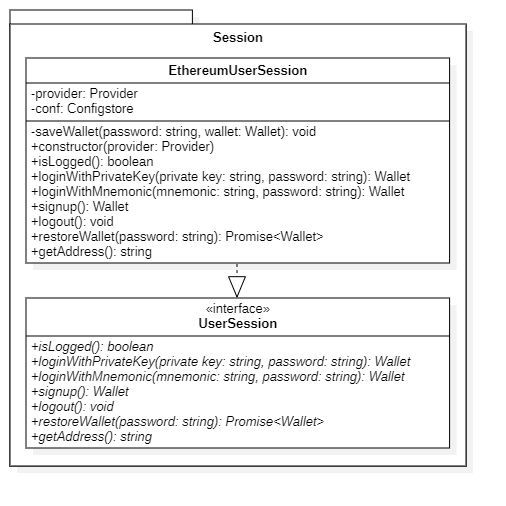
\includegraphics[width=0.5\linewidth]{diagrammi/etherless-cli/Session}
			\caption{Class diagram of the Session package.}
		\end{figure}
			
			\subsubsubsection{UserSession} 
			This interface defines the methods needed used to manage all the functions linked with the user session, like signup, login and logout. 
				\subsubsubsection*{Methods}
				\begin{itemize}
					\item \textbf{isLogged}: checks if the current user is logged;
					\item \textbf{loginWithPrivateKey}: provides the login procedure using private key;
					\item \textbf{loginWithMnemonicPhrase}: provides the login procedure using mnemonic phrase;
					\item \textbf{signup}: provides the procedure for the creation of a new user inside the system;
					\item \textbf{logout}: logs out the current user;
					\item \textbf{restoreWallet}: provide the procedure to obtain the local encrypted copy of user wallet;
					\item \textbf{getAddress}: retrieves the address of the current user.
				\end{itemize}
			
			\subsubsubsection{EthereumUserSession}
			Since the program uses the Ethereum network, we decided to create the class EthereumUserSession, that implements all methods of the UserSession interface for this network.
				\subsubsubsection*{Attributes}
					\begin{itemize}
						\item \textbf{provider}: provider that identifies the Ethereum network of interest; 
						\item \textbf{conf}: object used to save local configurations.
					\end{itemize}
				
				\subsubsubsection*{Methods}
				The class implements all the methods defined in UserSession interface. It also defines the following private methods: 
					\begin{itemize}
						\item\textbf{saveWallet}: creates a local crypted copy of the current wallet. 
					\end{itemize}
				
		\subsubsection{Contract} 
		This package is used to define all the classes and interfaces needed to interact with Ethereum blockchain and smart contracts. 
		\begin{figure} [h!]
			\centering
			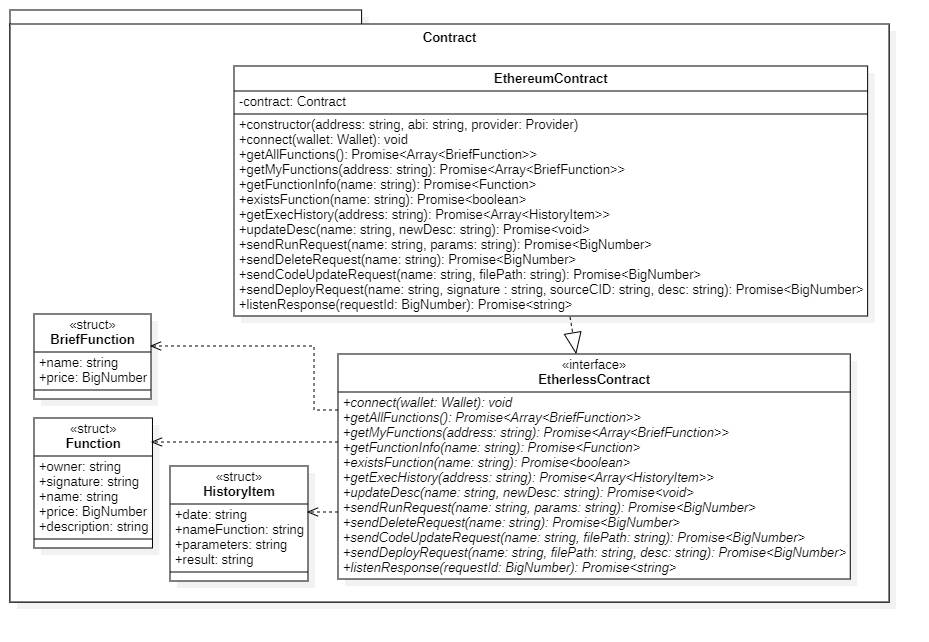
\includegraphics[width=0.75\linewidth]{diagrammi/etherless-cli/Contract}
			\caption{Class diagram of the Contract package.}
		\end{figure}
	
			\subsubsubsection{EtherlessContract}
			Interface that exposes methods for smart contract interaction and blockchain data elaboration. 	
			
				\subsubsubsection*{Methods}
					\begin{itemize}
						\item \textbf{connect}: connects a wallet to the contract instance;
						\item \textbf{getAllFunctions}: gets all functions that are successfully deployed inside the platform;
						\item \textbf{getMyFunctions}: returns the list of deployed function owned by the current user;
						\item \textbf{getFunctionInfo}: returns the details of a specific function;
						\item \textbf{existsFunction}: checks if a function exists inside \textit{Etherless} platform;
						\item \textbf{getExecHistory}: returns the list of past executions of the current user;
						\item \textbf{updateDesc}: updates the description of a function owned by the current user ;
						\item \textbf{sendRunRequest}: sends a function execution request;
						\item \textbf{sendDeleteRequest}: requests to delete a function owned by current user; 
						\item \textbf{sendCodeUpdateRequest}: requests to update the code of a function owned by the user; 
						\item \textbf{sendDeployRequest}: requests to deploy a new function; 
						\item \textbf{listenResponse}: listens the response of a previous request, independently from its type.
					\end{itemize}
		
			\subsubsubsection{EthereumContract} 
			We created the class EthereumContract that implements the EtherlessContract interface. In particular all its provided functionalities communicate with the \textit{Etherless-smart} module and fetch blockchain data. \\ To interact with the smart-contract it uses an instance of the Contract class, which is provided by the library \texttt{ethers.js}.
				\subsubsubsection*{Attributes}
					\begin{itemize}
						\item \textbf{contract}: instance of the Contract class provided by \texttt{ethers.js}. It is used to interact with a smart contract, and in particular with the \textit{Etheless-smart} module; 
					\end{itemize}
				
				\subsubsubsection*{Methods}
					The class implements all the methods defined in EtherlessContract interface.
	
	\subsection{UML}
	\begin{figure} [H]
		\centering
		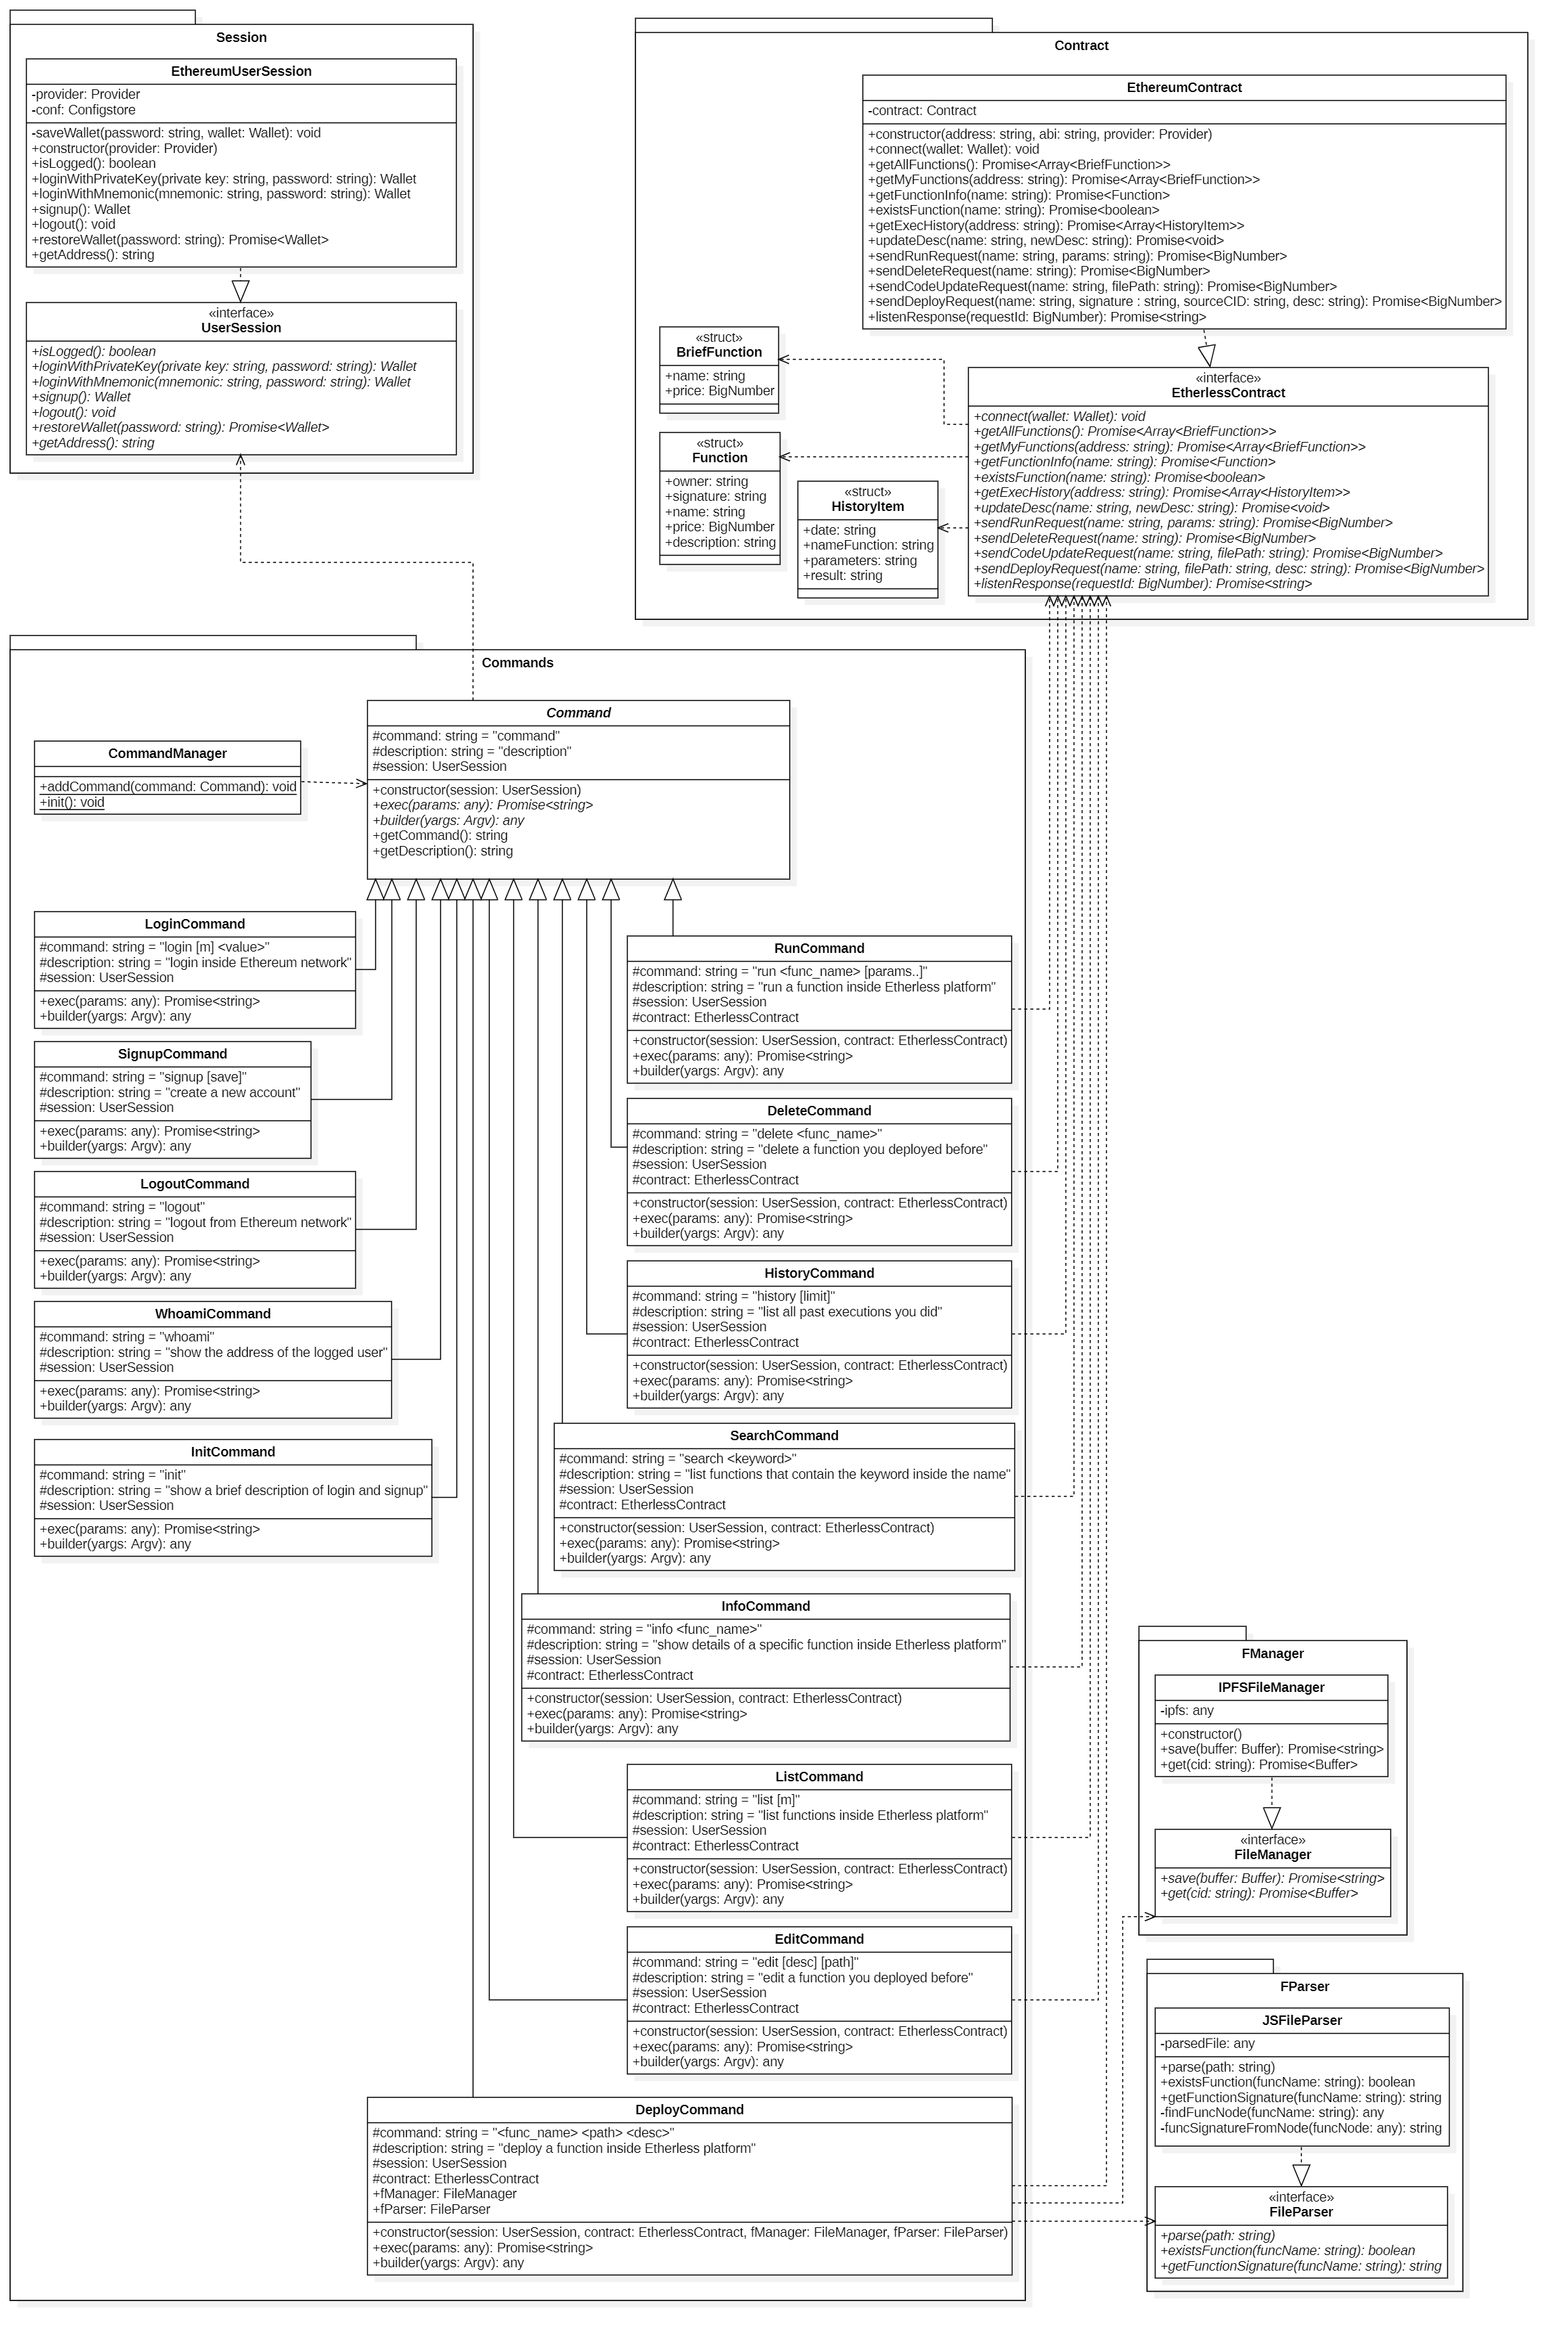
\includegraphics[width=0.85\linewidth]{diagrammi/etherless-cli/Classi}
		\caption{Class diagram of the Commands package.}
	\end{figure}
			
\subsection{Extensions}  
In order to allow the integration of new functionalities in the system, without heavy alterations of the existing architecture, various design choices were implemented.

\subsubsection{Parsing source file written in different languages}
Defining FileParser as an interface implies the possibility to expand the functionality of the product. In particular will be possibile to manage the parsing and then the deployment of source file written in different programming languages by simply defining new derived classes. 

\subsubsection{File management}
Defining FileManager as an interface implies the possibility to introduce different methods and protocols of file managing, by creating a specific class that implements this interface. 

\subsubsection{Introduction of new commands}
The development of Command as an abstract class, implies the possibility to provide the user new functionalities and CLI commands by creating new derivated classes. To correctly add the new command to the CLI, it will be necessary to use the class CommandManager.

\subsubsection{Other extensions}
Other components can be extended through re-definition. It will be necessary to implement the relative interfaces, which are:
\begin{itemize}
	\item \textbf{EtherlessContract Interface}: a high-level representation and handling of the main smart contract;
	\item \textbf{UserSession Interface:} provides functionalities to handle sessions.
\end{itemize}